\documentclass{article}

\usepackage[T1]{fontenc}     % Użycie poprawnego kodowania znaków
\usepackage[utf8]{inputenc}  % Kodowanie UTF-8
\usepackage[polish]{babel}   % Obsługa języka polskiego
\usepackage[left=3cm,right=3cm,top=3cm,bottom=3cm]{geometry}
\usepackage{graphicx}

% Otwarcie dokumentu
\title{Dokumentacja aplikacji do rozliczeń grupowych ŚciAppka}
\author{Łukasz Szenkiel}
\date{}

\begin{document}
	
\maketitle
\thispagestyle{empty}
\begin{center}
	\includegraphics[width=0.6\textwidth]{CWUPlogo.png}
\end{center}
	
\newpage
\begin{abstract}
Niniejszy dokument zawiera opis aplikacji do rozliczeń grupowych ŚciAppka, która umożliwia użytkownikom łatwe dzielenie się kosztami podczas wspólnych wyjazdów, zakupów i innych aktywności grupowych.
\end{abstract}
	
\section{Ogólny zarys programu}
Aplikacja ŚciAppka została zaprojektowana z myślą o użytkownikach, którzy często dzielą się kosztami w grupach. Każdy użytkownik może szybko i łatwo dodać swoje wydatki, a aplikacja automatycznie obliczy, ile każdy powinien zapłacić lub otrzymać. Program generuje raport, który jest zapisywany do pliku PDF i na potrzeby szkoleniowe MD.
	
\section{Funkcjonalność programu w diagramach UML}

W niniejszym projekcie kluczową rolę w wizualizacji struktury, przepływu pracy oraz interakcji użytkownika odegrało zastosowanie języka i narzędzia PlantUML. Wybór ten podyktowany był potrzebą efektywnego i spójnego przedstawienia aspektów systemu poprzez diagramy klas, czynności i przypadków użycia.\\
PlantUML stanowi innowacyjne podejście do tworzenia diagramów UML oraz innych wizualizacji technicznych, odchodząc od tradycyjnych graficznych edytorów na rzecz deklaratywnego języka tekstowego. Zamiast manualnego rozmieszczania elementów i łączeń, diagram definiowany jest poprzez precyzyjny opis składniowy, który następnie jest interpretowany przez silnik PlantUML w celu wygenerowania odpowiadającej mu reprezentacji graficznej. Wynikiem tego procesu są pliki obrazów w formatach takich jak PNG czy SVG, a także dokumenty PDF. Na potrzeby tej dokumentacji diagramy były eksportowane do formatu PGN.\\
Decyzja o implementacji PlantUML w procesie dokumentacji projektu przyniosła wymierne korzyści. Przede wszystkim, znacząco przyspieszyło to iteracyjny proces tworzenia i modyfikacji diagramów. Wszelkie zmiany w strukturze systemu czy logice działania mogły być szybko odzwierciedlone w diagramach poprzez prostą edycję opisu tekstowego, eliminując czasochłonne manualne poprawki graficzne. Co więcej, tekstowa reprezentacja diagramów naturalnie wpisuje się w praktyki kontroli wersji, umożliwiając śledzenie ewolucji wizualizacji w czasie i ułatwiając współpracę zespołu poprzez mechanizmy porównywania i scalania zmian.\\
Integracja PlantUML z wykorzystywanymi w projekcie narzędziami i środowiskami programistycznymi zapewniła płynny przepływ pracy. Opisy diagramów mogły być tworzone i zarządzane bezpośrednio w edytorach tekstu, a następnie automatycznie generowane do dokumentacji. Takie podejście gwarantuje również wysoką spójność wizualną wszystkich diagramów w projekcie, co przekłada się na lepszą czytelność i profesjonalizm dokumentacji.\\
W kontekście tego projektu, PlantUML okazał się nie tylko narzędziem do tworzenia statycznych obrazów, ale dynamicznym elementem procesu dokumentacyjnego, umożliwiającym efektywne komunikowanie złożonych koncepcji systemowych w sposób precyzyjny i zrozumiały. Wykorzystanie tego języka i narzędzia stanowiło świadomą decyzję mającą na celu podniesienie jakości i efektywności tworzonej dokumentacji.
	
\subsection{Diagram klas}
\begin{center}
	\includegraphics[width=0.7\linewidth]{diagram_klas.png}
\end{center}
Diagram klas przedstawia kluczowe klasy aplikacji ŚciAppka i ich relacje. Klasa Person reprezentuje uczestnika z informacjami o imieniu, wydatkach, długu i saldzie. Klasa Expense opisuje pojedynczy wydatek, wskazując nazwę, płacącego, kwotę, beneficjentów oraz informację, czy płacący jest również beneficjentem. Klasa Accounting reprezentuje pojedynczą transakcję rozliczeniową między dłużnikiem a wierzycielem. Klasa Calculation agreguje uczestników i wygenerowane rozliczenia. Relacje między klasami wskazują powiązania, takie jak płacący wydatek, beneficjenci wydatku oraz transakcje rozliczeniowe między osobami w ramach rozliczenia.
\subsection{Diagram przypadków użycia}
\begin{center}
	\includegraphics[width=1.1\linewidth]{diagram_przypadkow_uzycia.png}
\end{center}
Diagram przypadków użycia przedstawia interakcje między użytkownikiem a systemem ŚciAppka. Użytkownik może podać imiona uczestników, dodawać wydatki (z wyborem płacącego, kwoty i beneficjentów), rozliczać wydatki oraz wyświetlać wynik rozliczenia. System wykonuje obliczenia rozliczeniowe.
\subsection{Diagram czynności}
\begin{center}
	\includegraphics[width=0.7\linewidth]{diagram_czynnosci.png}
\end{center}
Diagram czynności przedstawia proces działania aplikacji ŚciAppka. Rozpoczyna się od wprowadzenia uczestników. Następnie, w pętli, użytkownik podaje szczegóły wydatków (cel, płacący, kwota, beneficjenci), aż zdecyduje się przejść do rozliczenia. Proces rozliczenia polega na iteracyjnym znajdowaniu osób z ujemnym i dodatnim bilansem oraz generowaniu przelewów wyrównujących różnice, aż wszystkie bilanse będą zerowe. Na końcu prezentowane jest rozliczenie.
	
\section{Wbudowane funkcje i klasy}
Aplikacja ŚciAppka wykorzystuje zarówno wbudowane funkcje i moduły języka Python, jak i zdefiniowane w ramach projektu klasy, do realizacji swojej funkcjonalności. Poniżej omówiono kluczowe elementy z obu tych kategorii.

\subsection{Wbudowane funkcje i moduły Pythona}

Aplikacja opiera się na kilku podstawowych wbudowanych funkcjach i modułach Pythona:
\begin{itemize}
\item input(): Funkcja ta służy do pobierania danych od użytkownika, np. imion uczestników, nazw wydatków, kwot. Jest to kluczowy element interakcji z użytkownikiem w trybie tekstowym.
\item print(): Funkcja ta jest wykorzystywana do wyświetlania informacji na konsoli, takich jak komunikaty dla użytkownika, dane o wydatkach i wynik rozliczenia.
\item float(): Funkcja ta służy do konwersji łańcucha znaków reprezentującego kwotę wydatku na liczbę zmiennoprzecinkową, co umożliwia wykonywanie operacji matematycznych.
\item int(): Funkcja ta służy do konwersji łańcucha znaków na liczbę całkowitą, na przykład przy pobieraniu numeru osoby z listy uczestników.
\item list(): Funkcja ta służy do tworzenia list, np. listy uczestników (team), listy wydatków (expenses) czy listy beneficjentów wydatku.
\item map(): Funkcja ta jest używana w połączeniu z int() i split() do konwersji listy łańcuchów znaków reprezentujących numery beneficjentów na listę liczb całkowitych.
datetime (moduł): Moduł ten jest używany do generowania znacznika czasowego w raporcie (funkcja datetime.now().strftime('%d-%m-%Y %H-%M-%S')), co pozwala na śledzenie, kiedy dany raport został wygenerowany.
\item os (moduł): Moduł ten jest używany do tworzenia katalogu na wyjściowe pliki (funkcja os.makedirs("out", exist\_ok=True)).
\item subprocess (moduł): Moduł ten służy do uruchamiania zewnętrznego procesu, jakim jest kompilator LaTeX (pdflatex).
\end{itemize}
\subsection{Klasy aplikacji}

W aplikacji ŚciAppka zdefiniowano następujące klasy, które reprezentują kluczowe elementy logiki biznesowej:
\begin{itemize}
\item Person: Klasa ta reprezentuje uczestnika rozliczenia.
\begin{itemize}
\item Atrybuty:
\begin{itemize}
\item name (str): Imię uczestnika.
\item expenses (float): Suma wydatków poniesionych przez uczestnika.
\item debt (float): Suma należności uczestnika (ile powinien zapłacić).
\item balance (float): Saldo uczestnika (różnica między poniesionymi wydatkami a należnościami).
\end{itemize}
\item Metody:
\begin{itemize}
\item \_\_init\_\_(self, name: str): Konstruktor klasy, inicjalizuje obiekt Person z podanym imieniem.
\item \_\_str\_\_(self): Metoda specjalna, zwraca łańcuch znaków reprezentujący obiekt Person, zawierający informacje o wydatkach, należnościach i saldzie.
\end{itemize}
\end{itemize}
\item Expense: Klasa ta reprezentuje pojedynczy wydatek.
\begin{itemize}
\item Atrybuty:
\begin{itemize}
\item name (str): Nazwa wydatku.
\item payer (Person): Osoba, która zapłaciła za wydatek.
\item amount (float): Kwota wydatku.
\item beneficiaries (List[Person]): Lista osób, które uczestniczą w kosztach wydatku.
\item is\_payer\_beneficiary (bool): Informacja, czy płacący jest również beneficjentem wydatku.
\item debt (float): Kwota przypadająca na jednego beneficjenta.
\end{itemize}
\item Metody:
\begin{itemize}
\item \_\_init\_\_(self, name: str, payer: Person, amount: float, beneficiaries: List[Person]): Konstruktor klasy, inicjalizuje obiekt Expense z podanymi danymi. Aktualizuje również informacje o wydatkach i saldzie płacącego oraz należnościach beneficjentów.
\item \_\_str\_\_(self): Metoda specjalna, zwraca łańcuch znaków reprezentujący obiekt Expense, zawierający informacje o nazwie wydatku, płacącym, kwocie i beneficjentach.
\end{itemize}
\end{itemize}
\item Accounting: Klasa ta reprezentuje pojedynczą transakcję rozliczeniową między dwoma uczestnikami.
\begin{itemize}
\item Atrybuty:
\begin{itemize}
\item refund\_giver (Person): Osoba, która ma dokonać zwrotu.
\item refund\_receiver (Person): Osoba, która ma otrzymać zwrot.
\item amount (float): Kwota zwrotu.
\end{itemize}
\item Metody:
\begin{itemize}
\item \_\_init\_\_(self, refund\_giver: Person, refund\_receiver: Person, amount: float): Konstruktor klasy, inicjalizuje obiekt Accounting i aktualizuje salda uczestników transakcji.
\end{itemize}
\end{itemize}
\item Calculation: Klasa ta odpowiada za przeprowadzenie obliczeń rozliczeniowych dla grupy osób.
\begin{itemize}
\item Atrybuty:
\begin{itemize}
\item team (List[Person]): Lista uczestników rozliczenia.
accountings (List[Accounting]): Lista transakcji rozliczeniowych.
\end{itemize}
\item Metody:
\begin{itemize}
\item \_\_init\_\_(self, team: List[Person]): Konstruktor klasy, inicjalizuje obiekt Calculation i przeprowadza obliczenia rozliczeniowe, tworząc listę obiektów Accounting.
\item \_\_str\_\_(self): Metoda specjalna, zwraca łańcuch znaków reprezentujący wynik obliczeń rozliczeniowych, czyli listę transakcji zwrotów.
\end{itemize}
\end{itemize}
\end{itemize}
\subsection{Relacje między klasami}

Klasy w aplikacji ŚciAppka są powiązane ze sobą w następujący sposób:
\begin{itemize}
\item Uczestnik (Person) może być płacącym (payer) za wiele wydatków (Expense).
\item Wydatek (Expense) ma jednego płacącego (payer) i wielu beneficjentów (beneficiaries), którzy są uczestnikami (Person).
\item Obliczenie (Calculation) zawiera listę uczestników (Person) i listę transakcji rozliczeniowych (Accounting).
\item Transakcja rozliczeniowa (Accounting) dotyczy dwóch uczestników (Person): osoby dokonującej zwrotu (refund\_giver) i osoby otrzymującej zwrot (refund\_receiver).
\end{itemize}
Te relacje pozwalają na modelowanie i przetwarzanie danych związanych z wydatkami grupowymi oraz generowanie rozliczeń między uczestnikami.

\section{Dalsze możliwości rozwoju programu}
Aplikacja ŚciAppka, w obecnej formie, realizuje podstawowe funkcje rozliczania wydatków grupowych. Istnieje jednak szereg możliwości dalszego rozwoju, które mogłyby znacząco zwiększyć jej użyteczność i funkcjonalność. Poniżej przedstawiono potencjalne kierunki rozwoju, skupiając się na prostszych do implementacji ulepszeniach oraz na zwiększeniu odporności programu na błędy.
\subsection{Rozszerzenia funkcjonalności}
\begin{itemize}
\item Interfejs graficzny (GUI): Opracowanie graficznego interfejsu użytkownika (np. przy użyciu biblioteki Tkinter, PyQt lub webowego frameworka Django/Flask) uczyniłoby aplikację bardziej intuicyjną i przyjazną dla użytkownika. Obecnie aplikacja działa w trybie tekstowym, co może być mniej wygodne dla niektórych użytkowników.
\item Baza danych: Zamiast przechowywania danych w pamięci, można by użyć bazy danych (np. SQLite) do trwałego przechowywania danych rozliczeń. Obecnie po zakończeniu działania programu dane są tracone, a baza danych pozwoliłaby na ich zapisywanie i odczytywanie między uruchomieniami.
\item Uwierzytelnianie użytkowników: Wprowadzenie prostego systemu uwierzytelniania użytkowników (np. logowanie z hasłem) umożliwiłoby oddzielenie danych różnych grup użytkowników i zwiększenie prywatności.
\item Możliwość uwzględnienia płatności przez większą liczbę osób: Obecnie aplikacja zakłada, że jeden wydatek ma jednego płacącego. Rozszerzenie funkcjonalności o możliwość rozdzielenia płatności za jeden wydatek na kilka osób (np. każdy płaci część rachunku w restauracji) uczyniłoby aplikację bardziej elastyczną.
\item Historia rozliczeń: Zapisywanie historii przeprowadzonych rozliczeń (np. w bazie danych lub plikach) pozwoliłoby na późniejsze przeglądanie i analizowanie wcześniejszych transakcji.
\end{itemize}

\subsection{Zabezpieczenia przed błędnymi danymi}
\begin{itemize}
\item Walidacja danych wejściowych: Wprowadzenie mechanizmów walidacji danych wejściowych od użytkownika jest kluczowe dla zapewnienia stabilności i poprawnego działania programu. Należy zweryfikować poprawność typów danych (np. czy kwota wydatku jest liczbą), zakresów wartości (np. czy numer osoby jest poprawny) oraz formatów (np. czy imiona uczestników są unikatowe).
\item Obsługa wyjątków: Zastosowanie bloków try-except pozwoli na eleganckie obsłużenie potencjalnych błędów, które mogą wystąpić podczas przetwarzania danych wejściowych, np. ValueError przy konwersji łańcucha znaków na liczbę. Zamiast przerywać działanie programu, można wyświetlić użytkownikowi komunikat o błędzie i poprosić o ponowne wprowadzenie danych.
\item Komunikaty dla użytkownika: W przypadku wykrycia niepoprawnych danych wejściowych, program powinien wyświetlać jasne i zrozumiałe komunikaty informujące użytkownika o rodzaju błędu i sposobie jego poprawienia.
\item Pętle wymuszające poprawne dane: Można użyć pętli while do wymuszania na użytkowniku wprowadzenia poprawnych danych. Program powinien pytać użytkownika o dane tak długo, aż zostaną one wprowadzone poprawnie.
\end{itemize}
\subsection{Usprawnienia techniczne}
\begin{itemize}
\item Refaktoryzacja kodu: Przeprowadzenie refaktoryzacji kodu mogłoby poprawić jego czytelność, modularność i wydajność.
\item Dokumentacja kodu: Uzupełnienie kodu o szczegółowe komentarze i dokumentację (np. w formacie Sphinx) ułatwiłoby jego zrozumienie i utrzymanie.
\end{itemize}
\section{Instrukcja obsługi wraz z najczęstszymi pytaniami}
\subsection{Instrukcja obsługi}
\begin{enumerate}
\item \textbf{Uruchomienie programu}
Aby uruchomić program ŚciAppka:
\begin{itemize}
\item zainstaluj Python (wersja 3.6+). Sprawdź: python --version lub python3 --version.
\item zainstaluj bibliotekę plantuml: pip install plantuml
\item zainstaluj LaTeX (np. MiKTeX lub TeX Live) i dodaj go do PATH, jeśli chcesz generować raporty PDF.
\item uruchom program: otwórz terminal, przejdź do katalogu z plikiem main.py i wykonaj: python main.py lub python3 main.py.
\end{itemize}
\begin{center}
\includegraphics[width=1\textwidth]{uruchomienie.png}
\end{center}

\item \textbf{Wprowadzenie uczestników rozliczenia}
Po uruchomieniu programu zostaniesz poproszony o podanie imion uczestników rozliczenia.
\begin{itemize}
\item wprowadź imiona: Wpisz imiona wszystkich osób, które brały udział w wydatkach, oddzielając każde imię przecinkiem.
\item unikatowe imiona: Pamiętaj, że imiona muszą być unikatowe. Program używa ich do identyfikacji uczestników.
\item format wprowadzenia: Upewnij się, że imiona są rozdzielone tylko przecinkami, bez dodatkowych spacji po przecinku (chyba że spacja jest częścią imienia).
\item potwierdź wprowadzenie: Po wprowadzeniu wszystkich imion naciśnij klawisz Enter.
\end{itemize}
\begin{center}
	\includegraphics[width=1\textwidth]{wprowadzenie_osob.png}
\end{center}

\item \textbf{Wprowadzenie wydatków}
Po wprowadzeniu uczestników program umożliwi dodawanie informacji o poszczególnych wydatkach. Dla każdego wydatku należy podać następujące dane:
\begin{itemize}
\item nazwa wydatku: Wpisz krótkie i zwięzłe określenie, co to był za wydatek (np. "Obiad w restauracji", "Bilety na koncert").
\item soba, która zapłaciła: Program wyświetli listę numerowaną wszystkich wprowadzonych uczestników. Wpisz numer osoby, która zapłaciła za dany wydatek.
\item kwota wydatku: Wpisz kwotę, jaką zapłaciła wskazana osoba. Użyj kropek (.) jako separatora dziesiętnego (np. 125.50).
\item osoby, które korzystały z wydatku (beneficjenci): Program ponownie wyświetli listę numerowaną uczestników. \item wpisz numery osób, które brały udział w danym wydatku, oddzielając je przecinkami. Jeśli w wydatku brali udział wszyscy, wpisz numer o jeden większy od liczby uczestników (np. jeśli uczestników jest 7, wpisz "8" dla wszystkich).
	\item potwierdź wprowadzenie: Po wprowadzeniu wszystkich imion naciśnij klawisz Enter.
\end{itemize}
\begin{center}
	\includegraphics[width=1\textwidth]{wprowadzenie_wydatku.png}
\end{center}

\item \textbf{Przejście do rozliczenia}
Po wprowadzeniu wszystkich wydatków, które chcesz uwzględnić w rozliczeniu, możesz przejść do obliczenia należności i wygenerowania raportu.
\begin{itemize}
	\item wybierz opcję rozliczenia: Po dodaniu wydatku program zapyta, czy chcesz dodać kolejny wydatek, czy przejść do rozliczenia.
	\item wprowadź "2": Aby przejść do rozliczenia, wprowadź cyfrę "2" i naciśnij Enter.
\end{itemize}
Po wprowadzeniu "2" i naciśnięciu Enter program rozpocznie obliczenia i wygeneruje raport rozliczeniowy. Raporty zostaną zapisane w różnych formatach w folderze o nazwie out, który zostanie utworzony w tym samym katalogu, w którym uruchamiasz program. 

\end{enumerate}
\subsection{Najczęstsze pytania (FAQ)}
\begin{enumerate}
\item \textbf{Do czego służy program ŚciAppka?}

Program ŚciAppka służy do rozliczania wydatków grupowych. Pomaga ustalić, kto komu i ile pieniędzy powinien zwrócić po wspólnych wydatkach, takich jak wyjścia do restauracji, podróże czy zakupy.

\item \textbf{Jakie dane wejściowe przyjmuje program?}

Program przyjmuje następujące dane wejściowe:
\begin{itemize}
\item listę imion uczestników rozliczenia.
\item szczegóły dotyczące każdego wydatku, w tym:
\item nazwę wydatku.
\item osobę, która zapłaciła za wydatek.
\item kwotę wydatku.
\item listę osób, które brały udział w wydatku (beneficjentów).
\end{itemize}
\item \textbf{Jak program definiuje "beneficjenta" wydatku?}

Beneficjentami wydatku są wszystkie osoby, które powinny ponieść część jego kosztów. Może to być cała grupa lub tylko jej część.

\item \textbf{Czy osoba, która zapłaciła za wydatek, może być również jego beneficjentem?}

Tak, osoba płacąca może być również beneficjentem wydatku. W takim przypadku jej udział w kosztach jest odpowiednio uwzględniany.

\item \textbf{Jak program oblicza, kto komu powinien zwrócić pieniądze?}

Program oblicza należności każdego uczestnika na podstawie wprowadzonych wydatków i beneficjentów. Następnie generuje listę transakcji zwrotów, minimalizując liczbę przelewów między uczestnikami.

\item \textbf{W jakiej formie prezentowane są wyniki rozliczenia?}

Program generuje raport w kilku formatach:

Tekstowy (wyświetlany na konsoli).
Markdown (.md)
LaTeX (.tex)
PDF (generowany z pliku .tex)
Diagram rozliczenia (w formacie .png i jako część raportu)
\item \textbf{Czy program generuje diagram rozliczenia?}

Tak, program generuje diagram rozliczenia w formacie PNG, który wizualizuje przepływ pieniędzy między uczestnikami.

\item \textbf{Czy program zapisuje dane rozliczenia?}

Obecna wersja programu nie zapisuje danych rozliczenia trwale. Po zakończeniu działania programu dane są tracone. ( Warto zaznaczyć, że w rozdziale o dalszym rozwoju sugerujemy dodanie bazy danych, żeby to zmienić )

\item \textbf{Jak uruchomić program?}

Program jest napisany w języku Python i wymaga jego zainstalowania. Aby go uruchomić, należy uruchomić skrypt Pythona (np. python main.py).

\item \textbf{Czy program wymaga zainstalowania dodatkowych bibliotek?}

Tak, program wymaga zainstalowania bibliotek plantuml i subprocess (który zazwyczaj jest częścią standardowej biblioteki Pythona), a także systemu LaTeX (np. TeX Live lub MiKTeX), jeśli chcemy generować raport w formacie PDF.
\end{enumerate}
\subsection{Prezentacja wyników przykładowego użycia}
\subsubsection{Raport Markdown}
\begin{center}
	\includegraphics[width=0.6\textwidth]{raportmd1.png}
\end{center}
\begin{center}
	\includegraphics[width=0.6\textwidth]{raportmd2.png}
\end{center}
\subsubsection{Diagram .png}
\begin{center}
	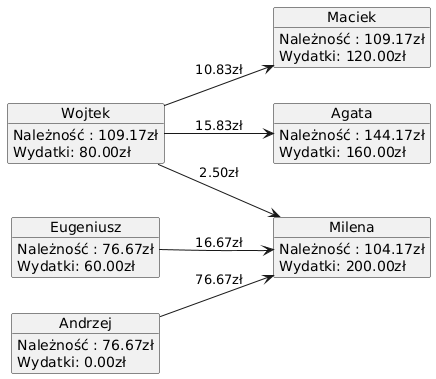
\includegraphics[width=0.6\textwidth]{diagram_rozliczenie.png}
\end{center}
\subsubsection{Raport PDF}
\begin{center}
	\includegraphics[width=0.6\textwidth]{raportPDF1.png}
\end{center}
\begin{center}
	\includegraphics[width=0.6\textwidth]{raportPDF2.png}
\end{center}
	
	
\end{document}
